%!TEX root = ../thesis.tex
%*******************************************************************************
%****************************** Second Chapter *********************************
%*******************************************************************************

\chapter{Lattice QCD}\label{chapter:LatticeQCD}

\ifpdf
    \graphicspath{{Chapter2/Figs/Raster/}{Chapter2/Figs/PDF/}{Chapter2/Figs/}}
\else
    \graphicspath{{Chapter2/Figs/Vector/}{Chapter2/Figs/}}
\fi
Since the first efforts to construct a non-perturbative approach to QCD in 1974\cite{Wilson:1974sk}, lattice QCD has developed over the past 40 years into a powerful tool used to probe the low-energy behaviour of the strong nuclear force. Rather than treat spacetime as a set of continuous axes, it is instead discretised into a finite set of points on a four-dimensional hypercube. This prescription allows for the explicit calculation of path integrals present in QCD, at the cost of introducing finite-spacing errors that must be systematically accounted for. In this chapter we will discuss the behaviour of QCD when spacetime is continuous (hereafter referred to as the continuum), and demonstrate how the transition can be made to a finite set of coordinates on a lattice. We will also describe the two choices of gauge used in this research, and how they are applied to the lattice. 

\section{QCD in the Continuum}
\subsection{Quarks and Gauge Invariance}
QCD is the gauge field theory that describes the interactions of quarks and gluons. Like all gauge theories, it has an internal symmetry group which the Lagrangian is invariant under. In the case of QCD there are three quark colours, which leads to the symmetry group being $SU(3)$, the group of $3\times 3$ unitary matrices of determinant 1 \footnote{This description is only true in the fundamental representation of the group, but this is the symmetry we observe in the Lagrangian and is a useful way to visualise the group symmetry.}. We can see this $SU(3)$ symmetry by inspecting the QCD quark Lagrangian
%
\begin{equation}
\mathcal{L} = \bar{\psi}(x)\,(i\slashed{\partial}-m)\,\psi(x)\,.
\label{eq:GlobalQuarkLagrangian}
\end{equation}
%
If we apply an $SU(3)$ transformation $\Omega$ to the colour indices of the quark, $\psi (x)$, and anti-quark, $\bar{\psi} (x)$, fields, we see that
%
\begin{align*}
\mathcal{L}\rightarrow\mathcal{L'}&=\bar{\psi}(x)\,\Omega^\dag\,(i\slashed{\partial}-m)\,\Omega\,\psi(x)\\
&= \bar{\psi}(x)\,(i\slashed{\partial}-m)\,\psi(x)\,\Omega^\dag\,\Omega\\
&= \bar{\psi}(x)\,(i\slashed{\partial}-m)\,\psi(x)\\
&= \mathcal{L}\, .
\end{align*}\\
%
Here we have made use of the unitarity property $U\,U^\dag = I$. If this symmetry were all we required then we would be done and our theory would be pleasantly simple. However, we find that we need our gauge symmetry to be \textit{local}; that is, we demand that our gauge transformation itself be a function of $x$\cite{peskin2018introduction}. In this case, we find that the derivative in Eq.~\ref{eq:GlobalQuarkLagrangian} results in a loss of $SU(3)$ symmetry. We can write an arbitrary $SU(3)$ gauge transformation as an exponential of the traceless, Hermitian group generators $\lambda_a$ (known as the Gell-Mann matrices) such that $\Omega=\exp\left(i\omega^a(x)\,\frac{\lambda_a}{2}\right)$. Using this form for $\Omega$, we find that under a gauge transformation the Lagrangian is now
%
\begin{align}
\mathcal{L}\rightarrow\mathcal{L'}&=\bar{\psi}(x)\,\Omega^\dag(x)\,(i\slashed{\partial}-m)\,\Omega(x)\,\psi(x)\nonumber\\
&=\bar{\psi}\,\Omega^\dag\left[-\frac{\lambda_a}{2}\,(\slashed{\partial}\,\omega^a(x))+i\,\Omega\,(\slashed{\partial}\,\psi)-m\,\Omega\,\psi\right]\nonumber\\
&= \mathcal{L}-\bar{\psi}\,\Omega^\dag\,\frac{\lambda_a}{2}(\slashed{\partial}\,\omega^a(x))\,\Omega\,\psi
\label{eq:LocalTrans}
\end{align}
%
To amend this, we introduce the notion of the gauge-covariant derivative
%
\begin{equation}
D_\mu = \partial_\mu - ig A_\mu(x)\, ,
\label{eq:CovariantDerivative}
\end{equation}
%
where $A_\mu(x)=A_\mu^a(x)\,\frac{\lambda_a}{2}$, and $A_\mu^a(x)$ are eight new `gauge potentials'. Making the substitution $\partial_\mu\rightarrow D_\mu$, we introduce a new term into the Lagrangian that gives rise to an interaction between our quark and gauge fields.
%
\begin{equation}
\mathcal{L}_\text{int} = g\,\bar{\psi}\,A_\mu(x)\,\psi
\label{eq:InteractingLagrangian}
\end{equation}
%
To preserve the gauge invariance of the Lagrangian, we need the gauge transformation property of Eq.~\ref{eq:InteractingLagrangian} to counteract the last term of Eq.~\ref{eq:LocalTrans}. Hence we require that
%
\begin{align}
g\,\bar{\psi}\,A_\mu(x)\,\psi \rightarrow g\,\bar{\psi}\,A_\mu(x)\,\psi + \bar{\psi}\,\Omega^\dag\,\frac{\lambda_a}{2}(\partial_\mu\,\omega^a(x))\,\Omega\,\psi\, .
\end{align}
%
Making use of the transformation properties of $\psi$ and $\bar{\psi}$, this implies that
%
\begin{equation}
A_\mu(x)\rightarrow \Omega\,A_\mu(x)\,\Omega^\dag - \frac{i}{g}\,(\partial_\mu\,\Omega)\,\Omega^\dag\, . 
\end{equation}\\
%

This transformation property can also be expressed in terms of the covariant derivative. Doing so, we find that
%
\begin{align*}
D_\mu\,\psi \rightarrow &\left(\partial_\mu -ig\,\Omega\,A_\mu(x)\,\Omega^\dag - (\partial_\mu\,\Omega)\,\Omega^\dag\right)\,\Omega\,\psi\\
&= (\partial_\mu\,\Omega)\,\psi + \Omega\,(\partial_\mu\,\psi) - ig\,\Omega\,A_\mu(x)\,\psi - (\partial_\mu\,\Omega)\psi\\
&=\Omega\,D_\mu\,\psi\, .
\end{align*}
%
And therefore
%
\begin{equation}
D_{\mu}\rightarrow\Omega\,D_\mu \Omega^\dag
\end{equation}
%
This result tells us that the covariant derivative of a quark field transforms in the same way as the quark field itself. The covariant derivative can then be thought of as a connection between two points that may have a different underlying gauge. For example, if we consider an infinitesimal translation in the quark field
%
\begin{equation*}
d\psi(x) = \psi(x+dx)-\psi(x)\, ,
\end{equation*} 
%
we note that the gauge at the point $x$ and at $x+dx$ in general will differ, so it doesn't make sense to compare the field values through the usual understanding of the derivative. Instead, the covariant derivative accounts for this underlying gauge structure, `transporting' the field from one position to another.\\

\subsection{Gluon Field}
Using local gauge invariance as a guide, we can now seek other gauge invariant terms to insert into the Lagrangian. If we consider the commutator of the covariant derivative, we have
%
\begin{align*}
[D_\mu,\, D_\nu]\rightarrow &[\Omega\,D_\mu\,\Omega^\dag,\,\Omega\,D_\nu\,\Omega^\dag]\\
&= \Omega\,D_\mu\, D_\nu\,\Omega^\dag - \Omega\,D_\nu\, D_\mu\,\Omega^\dag\\
&= \Omega\,[D_\mu,\,D_\nu]\,\Omega^\dag\, .
\end{align*}
%
We therefore define the gluon field strength tensor to be
%
\begin{equation}
F_{\mu\nu} = \frac{i}{g}\,[D_\mu,\, D_\nu]
\end{equation}
%
Expanding this definition, $F_{\mu\nu}$ may also be written
%
\begin{align}
F_{\mu\nu}=\partial_\mu A_\nu - \partial_\nu A_\mu - ig[A_\mu,\,A_\nu]
\label{eq:FieldStrengthTensor}
\end{align}
%
To obtain a gauge invariant quantity, we take the trace of the contracted field strength tensor. This allows us to make use of the cyclic property of the trace to obtain
%
\begin{align*}
\Tr(F_{\mu\nu}\,F^{\mu\nu})\rightarrow&-\frac{1}{g^2}\Tr\left(\Omega\,[D_\mu,\,D_\nu]\,\Omega^\dag\,\Omega\,[D^\mu,\,D^\nu]\,\Omega^\dag\right)\\
&=-\frac{1}{g^2}\Tr\left(\Omega^\dag\,\Omega\,[D_\mu,\,D_\nu]\,[D^\mu,\,D^\nu]\,\right)\\
&=\Tr(F_{\mu\nu}\,F^{\mu\nu})
\end{align*}
%
Thus we define the full gauge invariant QCD Lagrangian to be
%
\begin{equation}
\mathcal{L_{\text{QCD}}}=\bar{\psi}(x)\,(i\slashed{D}-m)\,\psi(x)-\frac{1}{2}\,\Tr(F_{\mu\nu}(x)\,F^{\mu\nu}(x))
\label{eq:QCDLagrangian}
\end{equation}\\

This gluon term is not the only gauge invariant quantity we could construct; for example, $\bar{\psi}\,\psi\,\bar{\psi}\,\psi$ is clearly gauge invariant. However, it turns out that there is a further condition that must be satisfied by each term in the Lagrangian; each term must be \textit{renormalisable}\cite{peskin2018introduction}. A complete discussion of renormalisation is unnecessary for this work, but renormalisability can be quickly summarised by looking at the dimensionality of each term in the Lagrangian. The Lagrangian must have units of $(\text{Energy})^4$, which in natural units is $(\text{mass})^4$ (hereafter referred to as just dimension 4). We therefore require that each term and its accompanying coupling constant give the same dimensionality. The fermion field has dimension $\frac{3}{2}$, the gauge potential has dimension 1 and $\partial_\mu$ has dimension 1. Then we see that the terms present in Eq.~\ref{eq:QCDLagrangian} have dimension
%
\begin{align*}
\text{D}[\bar{\psi}(x)\,\gamma^\mu\,\partial_\mu\,\psi(x)]&=\frac{3}{2}+1+\frac{3}{2}=4\\
\text{D}[\bar{\psi}(x)\,\gamma^\mu\,A_\mu\,\psi(x)]&=\frac{3}{2}+1+\frac{3}{2}=4\\
\text{D}[\bar{m\psi}(x)\,\psi(x)]&=1+\frac{3}{2}+\frac{3}{2}=4\\
\text{D}[F_{\mu\nu}\,F^{\mu\nu}] &= 2+2=4
\end{align*}
%
as required. This also tells us that the coupling constant $g$ is dimensionless. If a new gauge invariant term $h\bar{\psi}\,\psi\,\bar{\psi}\,\psi$ with coupling constant $h$ is introduced, we then require that $h$ have dimension $-2$. It turns out that if the dimensionality of the coupling constant is less than 0 then the term in non-renormalisable. This means that integrals involving this new term will diverge in such a way that they cannot be systematically be made finite through use of an ultraviolet cutoff, and hence they cannot form part of any physical theory. By applying the requirements of gauge invariance and renormalisability, it is apparent that Eq.~\ref{eq:QCDLagrangian} is the full QCD Lagrangian.

\subsection{Pure Gauge Action}
For the purpose of this research, we are interested in the behaviour of gluons in the absence of any quarks, and as such we need to develop a description of pure gauge fields. In the continuum, a pure gauge field has the Lagrangian\cite{ryder1996quantum}
%
\begin{equation}
\mathcal{L}_{\text{gluon}}=\frac{1}{2}\Tr(F_{\mu\nu}\,F^{\mu\nu})\, ,
\label{eq:GaugeLagrangian}
\end{equation}
%
which we observe to be the last term in Eq.~\ref{eq:QCDLagrangian}. This Lagrangian has the corresponding action
%
\begin{equation}
\mathcal{S}=\int~d^4x~\mathcal{L_\text{gluon}},
\label{eq:QCDAction}
\end{equation}
%
When considering the path integral formulation of a gauge field theory, integrals such as the generating functional,
%
\begin{equation}
\mathcal{Z} =\int \mathcal{D} A_\mu \exp\left(i\,\mathcal{S}\,[A_\mu(x)]\right),
\label{eq:GeneratingFunctional}
\end{equation}
%
and others of a similar form appear frequently. This integral closely resembles the partition function found in statistical mechanics, $Z_{\text{classical}}=\int d^3x\,d^3p\,\exp\left(-\beta\,H(x,p)\right)$, with the notable exception of the factor of $i$ in the exponential. From the statistical mechanics perspective, the $\exp(\ldots)$ term in the generating functional is a probability weighting for each `path' through gauge space. The factor of $i$ in Eq.~\ref{eq:GeneratingFunctional} results in an oscillatory weighting, rendering numerical simulations untenable. To ensure that the weight factor is purely real, it is necessary to perform a Wick rotation into Euclidean space\cite{Schafer:1996wv,Wilson:1974sk}
\begin{align*}
x_0\rightarrow -ix_0
\end{align*}
The generating functional now becomes 
\begin{equation}
\mathcal{Z}_{\text{Eucl}} =\int \mathcal{D} A_\mu \exp\left(-\mathcal{S}_{\text{Eucl}}\,[A_\mu(x)]\right).
\end{equation}
The Wick rotation also has the consequence of reducing the metric $g_{\mu\nu}$ to the identity, meaning that there is no longer any differentiation between covariant and contravariant tensors.\\


\section{Lattice Discretisation}
Within this framework, we can now consider discretising spacetime into a finite lattice with $N_s$ lattice sites in the spacial directions and $N_t$ sites in the time direction. Each lattice site is separated by a spacing $a$, resulting in a total lattice volume $V=(N_s\,a)^3\times N_t\,a$. This discretisation is shown in two dimensions in Fig.~\ref{fig:LatticeExample}. We also must impose periodic boundary conditions, such that $x+(N+1)a\hat{\mu}=x$.\\
%
\begin{figure}[h]
\centering
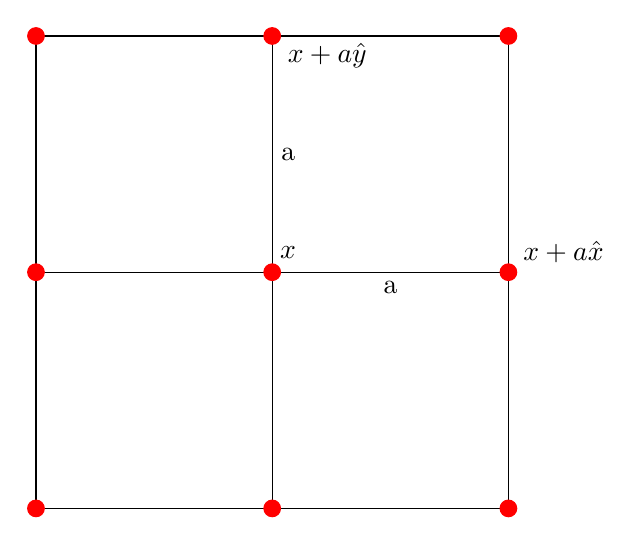
\begin{tikzpicture}
\draw [step=3cm] (-3-0.0001,-3-0.0001) grid (3,3);
\draw plot[mark=*,mark size = 3pt,mark options={color=red}] coordinates {(-3,-3)(0,-3)(0,0)(-3,0)(-3,3)(0,3)(3,3)(3,0)(3,-3)};
\node at (1.5,-0.2) {a};
\node at (0.2,1.5) {a};
\node at (0.2,0.25) {$x$};
\node at (3.7,0.25) {$x+a\hat{x}$};
\node at (0.7,2.75) {$x+a\hat{y}$};
\end{tikzpicture}
\caption{\label{fig:LatticeExample}An example of a 2D lattice with lattice spacing $a$. If we have a position $x$ then we can define $x+a\hat{\mu}$ to represent the next lattice site in the $\hat{\mu}$ direction.}
\end{figure}
%

When spacetime is discretised, it becomes necessary to consider derivatives as finite differences and integrals as finite sums.
\begin{align*}
\partial_\mu\,f(x)&\rightarrow \frac{f(x+a\hat{\mu})-f(x)}{a}\\
\int d^4x~f(x) &\rightarrow a^4\sum_x \,f(x)
\end{align*}
For example, we can construct the lattice form of Eq.~\ref{eq:FieldStrengthTensor} as
%
\begin{equation}
F_{\text{Lat}}^{\mu\nu}(x) = \frac{A_\nu(x+a\hat{\mu})-A_\nu(x)}{a}-\frac{A_\mu(x+a\hat{\nu})-A_\mu(x)}{a}-ig[A_\mu(x),\,A_\nu(x)].
\label{eq:DiscreteFST}
\end{equation}
%
The notation $A_\nu(x+a\hat{\mu})$ denotes the field $A_\nu$ located at the site one lattice spacing in the $\hat{\mu}$ direction from $x$. We could continue to reformulate our lattice theory by imposing this method of discretisation, and indeed this is historically how the lattice framework was constructed\cite{Wilson:1974sk}. However, it is useful to instead formulate our lattice theory in terms of the gauge {\it links}. Analogous to how we introduced the covariant derivative to compensate for the fact that the quark field at infinitesimally different points in space has a different underlying gauge, we now want to have a mechanism for comparing quark fields at some finite separation. This requires us to solve the parallel transport equation of our gauge field~\cite{Bing:1999ee}
%
\begin{equation}
\frac{dx_\mu(t)}{dt}\,D_\mu U(x_\mu(t))=0,~t\in [0,1]\, ,
\end{equation}
%
where $U(x_\mu(t))$ is an $SU(3)$ element satisfying $U(x_\mu(0))=I$. Using the explicit parametrisation $x_\mu = y_\mu+a\,t\,\hat{\sigma}$, where $y_\mu$ is a fixed position and $\sigma$ is a fixed direction, we have
\begin{align*}
&a\,\delta^\sigma_\mu\, (\partial_\mu-igA_\mu)\,U(y_\mu+a\,t\,\hat{\sigma})=0\\
&a\partial_\sigma\, U(y_\mu+a\,t\,\hat{\sigma}) = iag\, A_\sigma\,U(y_\mu+a\,t\,\hat{\sigma})\\
&\frac{\partial}{\partial t}U(y_\mu+a\,t\,\hat{\sigma}) = ig\,A_\sigma\, U(y_\mu+a\,t\,\hat{\sigma})\, .
\end{align*}
This is precisely the differential equation solved by the path-ordered exponential, so we find for each direction the gauge links
\begin{equation}
U_\mu(x) = \mathcal{P}\exp\left(ig\int_x^{x+a\hat{\mu}}dx'\,A_\mu(x')\right)\, .
\label{eq:GaugeLink}
\end{equation}
From this definition we also see that we can write the gauge link in the opposite direction, i.e. from $x+a\hat{\mu}$ to $x$, as
\begin{align*}
\mathcal{P}\exp\left(ig\int^x_{x+a\hat{\mu}}dx'\,A_\mu(x')\right) &= \mathcal{P}\exp\left(-ig\int_x^{x+a\hat{\mu}}dx'\,A_\mu(x')\right)\\
&=U^\dag_\mu(x)\, .
\end{align*}
These gauge links have the simple gauge transformation property~\cite{Lepage:1998dt}
\begin{equation}
U_\mu\rightarrow \Omega(x)\,U_\mu(x)\,\Omega^\dag(x+a\hat{\mu})\, .
\end{equation}
Making use of this gauge transformation property, we can construct gauge invariant Wilson loops by taking the product of the $U_\mu$'s around a closed loop. The simplest such loop, the $1\times 1$ square, is called the \textit{plaquette}, and is defined as
\begin{equation}
P_{\mu\nu}(x) = U_\mu(x)\,U_\nu(x+a\hat{\mu})\, U_\mu^\dag(x+a\hat{\nu})\, U_\nu^\dag(x)\, .
\label{eq:Plaquette}
\end{equation}

Taking the trace of this loop we see that by the cyclic property of the trace this is gauge invariant
\begin{align*}
\Tr\left(P_{\mu\nu}(x)\right)\rightarrow& \Tr \left(\Omega(x)\,U_\mu(x)\Omega^\dag(x+a\hat{\mu})\,\Omega(x+a\hat{\mu})\,U_\nu(x+a\hat{\mu})\,\Omega^\dag(x+a\hat{\mu}+a\hat{\nu})\right.\\
&~~~~~\left.\Omega(x+a\hat{\mu}+a\hat{\nu})\,U_\mu^\dag(x+a\hat{\nu})\,\Omega^\dag(x+a\hat{\nu})\,\Omega(x+a\hat{\mu})\, U_\nu^\dag(x)\,\Omega^\dag(x)\right)\\
=&\Tr\left(P_{\mu\nu}(x)\right)\, .
\end{align*}

We now return to the lattice formulation, making use of the gauge links to define our quantities of interest. Firstly, we approximate our gauge links using a midpoint approximation, such that
\begin{equation}
U_\mu^\text{lat}(x) = \exp\left(iag\, A_\mu\left(x+\frac{a}{2}\hat{\mu}\right)\right)\, .
\label{eq:GaugeLinkLat}
\end{equation}
From this definition, we can also recover the the midpoint gauge potential~\cite{Leinweber:1998im,Alles:1996ka}
\begin{equation}
A_\mu\left(x+\frac{a}{2}\hat{\mu}\right) = \frac{1}{2iag}\left(U_\mu(x) - U_\mu^\dag(x)\right) - \frac{1}{6iag}\Tr\left(U_\mu(x) - U_\mu^\dag(x)\right)I + \mathcal{O}(a^2)\, .
\label{eq:GaugePotentialLat}
\end{equation}
We then note that we can write $F_{\mu\nu}$ in terms of the plaquette by Taylor expanding Eq.~\ref{eq:Plaquette} to obtain~\cite{Gupta:1997nd}
%
\begin{equation}
P_{\mu\nu} = I+ia^2g\, F_{\mu\nu} - \frac{a^4 g^2}{2}F_{\mu\nu}F^{\mu\nu} +\mathcal{O}(a^6)\, ,
\end{equation} 
%
and hence
%
\begin{align}
a^4\Tr\left(F_{\mu\nu}F^{\mu\nu}\right) = \frac{2}{g^2}\Tr\left(I-\frac{1}{2}\left(P_{\mu\nu}+P_{\mu\nu}^\dag\right)\right)\, .
\end{align}
%
We have now arrived at a definition of the contracted field strength tensor that can be used to define our lattice action. As we sum over the 6 unique plaquettes, we take into account a factor of $2$ to arrive at the definition 
%
\begin{equation}
\mathcal{S}_\text{lat} = \frac{6}{g^2}\sum_x\,\sum_{\mu<\nu} \frac{1}{3}\Tr\left(I-\frac{1}{2}\left(P_{\mu\nu}+P_{\mu\nu}^\dag\right)\right)\, .
\end{equation}
%
To remove higher order errors from the lattice action, it is possible to take into account terms containing larger Wilson loops, following procedure similar to the one outlined above~\cite{Alford:1995hw,Symanzik:1983dc,Symanzik:1983gh}. For the purpose of this work, the gauge fields were generated using the $\mathcal{O}(a^2)$-improved L\"uscher and Weisz action~\cite{Luscher:1984xn}, which consists of a linear combination of $1\times 1$ plaquettes and $2\times 1$ rectangles.\\

This lattice framework provides the tools necessary to explicitly calculate quantities of interest. Firstly, the gauge links are generated by monte-carlo methods, using $\exp\left(-\mathcal{S}\right)$ as a probability weighting for a given configuration. Once these configurations are generated, gauge fixing can be performed (Sec.~\ref{sec:LandauGauge}, \ref{sec:MCG}), and quantities such as the gluon propagator (Chapter~\ref{chapter:GluonPropagator}) can be obtained.

\section{Gauge Fixing}
The choice of gauge is crucial when performing calculations on the lattice, or more generally in any gauge field theory calculation. There are two choices of gauge relevant to this study: Landau gauge and maximal centre gauge. Maximal centre gauge is best explored in the context of centre vortices, and will therefore be detailed in chapter~\ref{sec:MCG}, however the Landau gauge fixing condition provides a good introduction to the gauge fixing procedure, and as such will be described here.

\subsection{Landau Gauge}\label{sec:LandauGauge}

In the continuum, Landau gauge corresponds to imposing the condition
\begin{equation}
\partial_\mu A^\mu = 0\, .
\label{eq:LandauGaugeCont}
\end{equation}
%
On the lattice, we can approximate this condition by imposing
\begin{equation}
\Delta(x) = \sum _ { \mu } A _ { \mu } \left( x + \frac{a}{2}\hat { \mu } \right) - A _ { \mu } \left( x-\frac{a}{2}\hat { \mu } \right) = 0\, .
\label{eq:LandauGaugeLat}
\end{equation}
Here the fact that we have defined the lattice gauge potential to be at the midpoint of the link produces an improved continuum limit when we consider Eq.~\ref{eq:LandauGaugeLat} in momentum space~\cite{Alles:1996ka}. Performing a discrete Fourier transform, we see that
%
\begin{align}
\Delta(p) &= \sum_x \Delta(x) e^{-i\,p\cdot x} \nonumber\\
&=\sum_{x,\,\mu} e^{-i\,p\cdot x} \left(A _ { \mu } \left( x + \frac{a}{2}\hat { \mu } \right) - A _ { \mu } \left( x-\frac{a}{2}\hat { \mu } \right)\right) \nonumber\\
&= \sum_{x,\,\mu} e^{i\,p\cdot\frac{a}{2}\hat{\mu} }\,e^{-i\,p\cdot\left(x+\frac{a}{2}\hat{\mu} \right)}A _ { \mu } \left( x + \frac{a}{2}\hat { \mu } \right) - e^{-i\,p\cdot\frac{a}{2}\hat{\mu} }\,e^{-i\,p\cdot\left(x-\frac{a}{2}\hat{\mu} \right)}A _ { \mu } \left( x - \frac{a}{2}\hat { \mu } \right) \nonumber\\
&= \sum_\mu \left(e^{i\,p\cdot\frac{a}{2}\hat{\mu} } - e^{-i\,p\cdot\frac{a}{2}\hat{\mu} }\right) A_\mu(p) \nonumber\\
&=\sum_\mu 2i\sin\left(\frac{a}{2} p_\mu\right)A_\mu(p) = 0\, .
\label{eq:LandauGaugeLatP}
\end{align}
%
This is to be compared to the momentum space Landau gauge condition that can be obtained from the gauge potential defined on the lattice sites, which has the form~\cite{Alles:1996ka}
%
\begin{equation}
\sum _ { \mu } \left[ \left( \cos (a\,p _ { \mu }) - 1 \right) - i \sin (ap _ { \mu }) \right] A _ { \mu } ^ { \prime } ( p ) = 0\, .
\label{eq:LandauGaugeLatBad}
\end{equation}
%
In the limit as $a\rightarrow 0$, it can be seen that Eq.~\ref{eq:LandauGaugeLatP} exhibits
$\mathcal{O}(a^2)$ improvement, whereas Eq.~\ref{eq:LandauGaugeLatBad} has only $\mathcal{O}(a)$ improvement.\\

The Landau Gauge condition is imposed on the Lattice by finding extrema of the functional~\cite{Bonnet:1999mj}
%
\begin{equation}
\mathcal{F} =  \frac{4}{3}\mathcal{F}_1 - \frac{1}{12u_0}\mathcal{F}_2\, ,
\label{eq:LGFunctional}
\end{equation}
%
where
%
\begin{align*}
\mathcal{F}_1 &= \sum _ { \mu , x } \frac { 1 } { 2 } \operatorname { Tr } \left\{ U _ { \mu } ^ { G } ( x ) + U _ { \mu } ^ { G } ( x ) ^ { \dagger } \right\}\\
\mathcal{F}_2 &= \sum _ { \mu , x } \frac { 1 } { 2 } \operatorname { Tr } \left\{ U _ { \mu } ^ { G } ( x ) U _ { \mu } ^ { G } ( x + a\hat { \mu } ) + \mathrm { h.c. } \right\}\\
u_0 &= \left(\frac{1}{3}\operatorname{ Re } \Tr\langle U_\text{pl} \rangle\right)^{\frac{1}{4}}\, .
\end{align*}
%
The $u_0$ term contains the average value of the gauge links in the lattice, $\langle U_\text{pl} \rangle$, necessary to restore the continuum limit of $\mathcal{F}_2$ as $a\rightarrow 0$~\cite{Lepage:1992xa}. We also explicitly write $U^G_\mu$ to indicate that we are considering gauge links under as-yet unknown gauge transformation 
%
\begin{equation}
\Omega(x) = \exp\left( i\omega^a(x)\frac{\lambda_a}{2} \right)
\end{equation}
%
It becomes apparent why this we seek the extrema of this particular functional when we take the functional derivative with respect to the free parameters of the gauge transformation, $\omega^a(x)$.
%
\begin{equation}
\frac { \delta \left\{ \frac { 4 } { 3 } \mathcal { F } _ { 1 } - \frac { 1 } { 12 u _ { 0 } } \mathcal { F } _ { 2 } \right\} } { \delta \omega ^ { a } ( x ) } = g a ^ { 2 } \sum _ { \mu } \operatorname { Tr } \left\{ \left[ \partial _ { \mu } A _ { \mu } ( x ) - \frac { 4 } { 360 } a ^ { 4 } \partial _ { \mu } ^ { 5 } A _ { \mu } ( x ) + \mathcal { O } \left( a ^ { 6 } \right) \right] \frac{\lambda^a}{2} \right\} + \mathcal { O } \left( g ^ { 3 } a ^ { 4 } \right)
\label{eq:LGFunctionalDeriv}
\end{equation}
%
If Eq.~\ref{eq:LGFunctionalDeriv} is at an extrema, then 
%
\begin{equation*}
\sum_\mu \partial_\mu A_\mu(x) = \sum_\mu \frac{4}{360}a^4 \partial_\mu^5\,A_\mu(x) + \mathcal{O}(a^6)+\mathcal{O}(g^3a^4)\, .
\end{equation*}
%
Hence at order $\mathcal{O}(a^4)$, finding the extrema of Eq.~\ref{eq:LGFunctionalDeriv} is equivalent to satisfying the continuum Landau gauge condition, Eq.~\ref{eq:LandauGaugeCont}.

\section{Lattice units}

In the previous section, we have explicitly detailed how a variety of lattice quantities are constructed. For clarity, it is useful to remove extraneous constants by utilising so-called `lattice units'. Transforming to lattice units is done by setting $a=g=1$, which gives the following transformations
%
\begin{align*}
A_\mu \left( x+\frac{a}{2}\hat{\mu} \right)&\rightarrow A_\mu \left(x+\frac{\hat{\mu}}{2} \right)\\
U_\mu(x) &\rightarrow \exp\left( i A_\mu \left(x+\frac{\hat{\mu}}{2}\right)\right)\\
P_{\mu\nu}(x) &\rightarrow U_\mu(x)\,U_\nu(x+\hat{\mu})\, U_\mu^\dag(x+\hat{\nu})\, U_\nu^\dag(x)
\end{align*}
%\begin{landscape}
%
%\section*{Subplots}
%I can cite Wall-E (see Fig.~\ref{fig:WallE}) and Minions in despicable me (Fig.~\ref{fig:Minnion}) or I can cite the whole figure as Fig.~\ref{fig:animations}
%
%
%\begin{figure}
%  \centering
%  \begin{subfigure}[b]{0.3\textwidth}
%    \includegraphics[width=\textwidth]{TomandJerry}
%    \caption{Tom and Jerry}
%    \label{fig:TomJerry}   
%  \end{subfigure}             
%  \begin{subfigure}[b]{0.3\textwidth}
%    \includegraphics[width=\textwidth]{WallE}
%    \caption{Wall-E}
%    \label{fig:WallE}
%  \end{subfigure}             
%  \begin{subfigure}[b]{0.3\textwidth}
%    \includegraphics[width=\textwidth]{minion}
%    \caption{Minions}
%    \label{fig:Minnion}
%  \end{subfigure}
%  \caption{Best Animations}
%  \label{fig:animations}
%\end{figure}
%
%
%\end{landscape}
